\chapter[Capítulo 6. Pruebas de Funcionamiento]{Pruebas de Funcionamiento}

\section{Simulador SAE J1939}

El Au-SAE J1939 simulador Ver 2.00A es un dispositivo capaz de proveer la mayoría de las señales de la norma SAE J1939. Una topología de red típica SAE J1939 se ilustra en la \textbf{Figura \ref{TPSAE}}.

\begin{figure}[H]
	\centering
		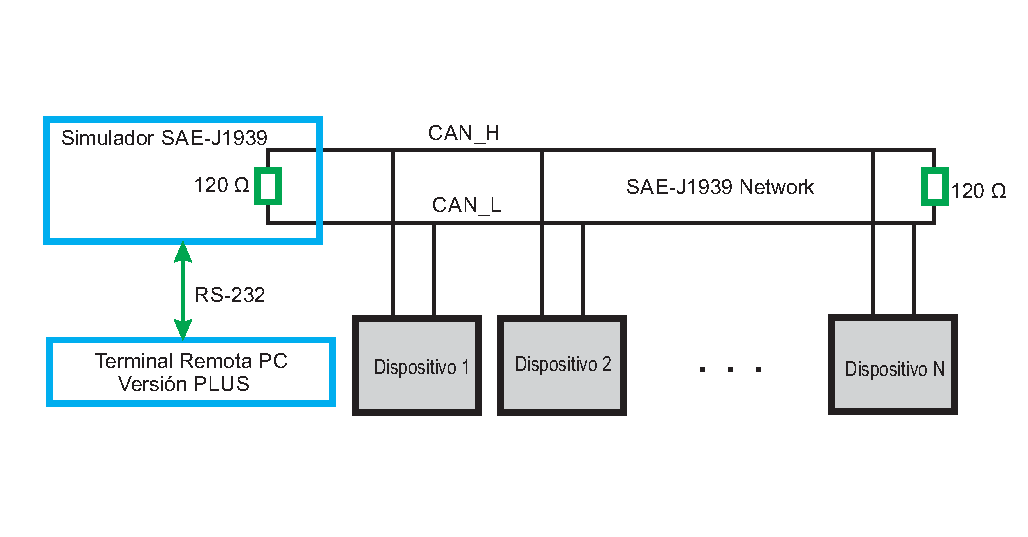
\includegraphics[width=0.8\textwidth]{./Cap6imagen/EjemploSimulador.pdf}
	\caption[Topología de Red SAE J1939.]{Topología de Red SAE J1939.\textbf{ Fuente:} \cite{UserM}.}
	\label{TPSAE} % Etiqueta para la referencia.
\end{figure}

Existen 6 ediciones del simulador  Gen II SAE J1939 de la \textbf{Figura \ref{Sim}}, que son proporcionados por Electrónica Au Grup para satisfacer las necesidades según los diferentes usuarios: 

\begin{figure}[H]
	\centering
		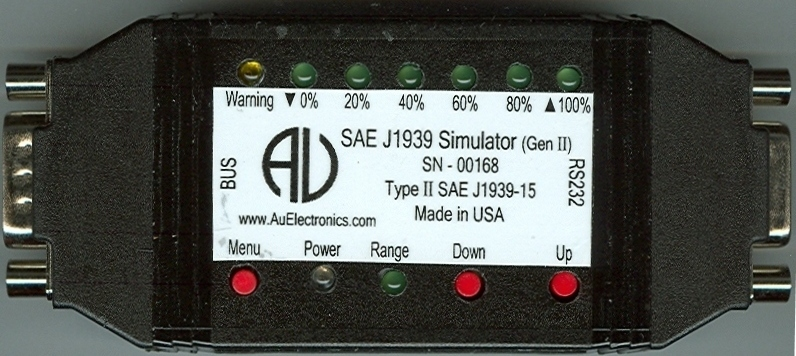
\includegraphics[width=0.8\textwidth]{./Cap6imagen/Simulador.png}
	\caption[Simulador BUS CAN SAE J1939.]{Simulador BUS CAN SAE J1939.\textbf{ Fuente:} \cite{UserM}.}
	\label{Sim} % Etiqueta para la referencia.
\end{figure}


\begin {itemize}
  
    \item Simulador Gen II  SAE-J1939  - Engine Basic Edition
	\item Simulador Gen II  SAE-J1939  - Engine Basic Plus Edition
	\item Simulador Gen II  SAE-J1939  - Engine Premium Edition
	\item Simulador Gen II  SAE-J1939  - Engine Premium Plus Edition
	\item Simulador Gen II  SAE-J1939  - Vehicle Platinum Edition
	\item Simulador Gen II  SAE-J1939  - Vehicle Platinum Plus Edition

\end{itemize}

Las ediciones "Plus" tienen todas las funciones de las ediciones "no-Plus", además de un programa de ordenador de terminal remota que puede ser utilizado para controlar y visualizar los datos SAE J1939 en la pantalla del PC. Además un conjunto de herramientas de gestión de licencias proporciona la capacidad de actualizar el simulador de edición básica de edición premium / platino. "Non-Plus" edición es capaz de ser actualizado a las ediciones "Plus".

\begin{itemize}
\item Engine Basic Edition: Genera la mayor parte de los datos básicos del motor de manera "Estática" o "Dinámica". Los dos botones (Up y Down) se utilizan para ajustar la salida de datos del simulador en el "modo estático" o en el "modo dinámico" respectivamente.En el "modo dinámico" los datos cambian de forma automática según los intervalos de valores estándares para el SAE  J1939. Los LEDs indican el valor del paso de control de la señal de salida, tiene un zumbador que indica el cambio de estado del simulador e indica el encendido del mismo.
\item Motor Premium Edition:
Incluye todas las funciones del motor Basic Edition e Incluye características premium de diagnosis del vehículo denominado DM1 (Diagnostics Message 1, por sus siglas en inglés),  DM2 y DM3 los cuales son parámetros que diagnostican el estado del vehículo.

\item Vehicle Platinum Edition: Incluye todas las funciones del motor Premium Edition, además incluye funciones que involucran la red interna del vehículo,  Señales relacionadas con el ABS (Antiblockiersystem), señales relacionadas con la transmisión y señales relacionadas con la Configuración del motor, \cite{UserM}.

\end{itemize}

\subsection {Principales Características del Simulador}

\begin{itemize}

\item Contiene una resistencia de carga interna 120 ohmios para montar una red BUS CAN.
\item Protección con  TVS (Transient Voltage Suppressor, por sus siglas en ingles) para protección contra altos niveles de tensión. 
\item Tamaño compacto.
\item 9 Indicadores LED: Encendido, Rando y Advertencia, HASTA 100\%, frente a 0\%, 80\%, 60\%, 40\%, 20\%, el  LED parpadeará cuando se selecciona uno de estos seis valores especificados.
\item Color de la carcasa: Negro 
\item 1 Zumbador
\item 3 botones: MENU, DOWN, UP, la señal J1939 se puede ajustar a través de estos pulsadores.
\item 1 interfaz RS232 para la actualización de software, gestión de licencias y control remoto.
\item 1 conector DB9 macho para la alimentación y la conexión CANH - CANL.
\item Fuente de alimentación: 9 a 12 VDC, 250mA máximo.
\item Temperatura de funcionamiento: -20$^{\circ}$C a 85$^{\circ}$C

\end{itemize}

\subsection{Modo de Funcionamiento}

Las simulaciones pueden ser operadas con sólo el control de los 3 botones presentes en el equipo. Con la configuración guiada por estos botones se genera una señal SAE J1939 para su uso en desarrollos de sistemas BUS CAN para camiones.

El equipo debe conectarse a una fuente externa entre 9-12 V. La alimentación se realiza con los pines 1 (Tierra) y 5 (Potencial positivo), la conexión del BUS CAN tanto CANH como CANL se realiza en los pines 6 y 7 como se muestra en la \textbf{Figura \ref{DB9}}.  El indicador LED de encendido se ilumina y al estar listo el equipo emite un sonido a través del zumbador, entonces el simulador Au SAE J1939 empieza a funcionar en el modo (estático o dinámico) guardado en la última vez de su funcionamiento.

\begin{figure}[H]
	\centering
		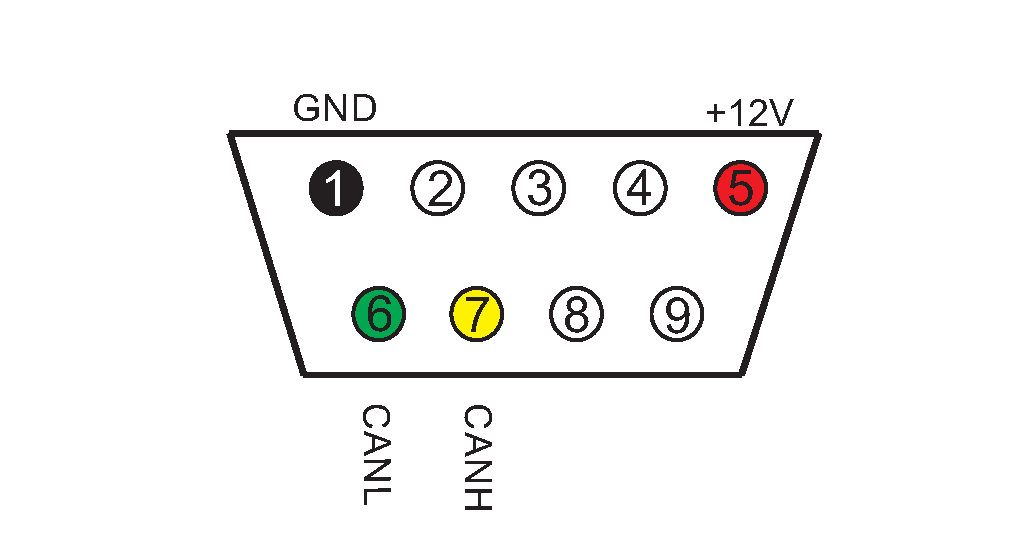
\includegraphics[width=0.8\textwidth]{./Cap6imagen/SimDb9.pdf}
	\caption[Conector DB9 macho BUS CAN.]{Conector DB9 macho BUS CAN.\textbf{ Fuente:} \cite{UserM}.}
	\label{DB9} % Etiqueta para la referencia.
\end{figure}

El modo estático genera una señal SAE J1939 constante, los  dos pulsadores (Up y Down) se utiliza para cambiar las salidas de datos mediante la decisión del usuario. En el modo dinámico todos los datos SAE-J1939 cambian automáticamente sin que el rango de valores sea intervenido por el usuario del equipo. Para Pasar de un modo de funcionamiento a otro se presiona los botones MENU y UP al mismo tiempo durante más de 1 segundo, es decir, para cambiar entre el modo dinámico y el modo estático. Una vez realizado, la confirmación del cambio se detecta con un zumbido del equipo.

En el modo estático el botón Down se utiliza para decrementar los valores de las señales SAE-J1939 presentes en las salidas del BUS CAN. Los leds muestran el descenso de las señales de manera porcentual, de la misma manera el botón Up se utiliza para aumentar los valores de las señales SAE-J1939 y los leds muestran el aumento de las señales de manera porcentual. la manera de cambiar entre estos dos modos se realiza presionando al mismo tiempo los botones MENÚ y UP por más de un segundo, de esta manera se intercala entre los modos de funcionamiento estático y dinámico. Un pitido largo será oído para reflejar la entrada de la tecla MENU y UP.

A modo de resumen se indica las funciones básicas de los botones:
\begin{itemize}
\item Botón DOWN: permite disminuir todos los datos simulados hasta que alcanza el valor más bajo.
 \item botón UP: permite aumentar todos los datos simulados hasta que alcanza el valor más alto.
\item botón MENÚ: activa y desactiva el DM1, esta opción no esta disponible en la versión básica.
\item Mantener presionado el botón MENÚ cuando se enciende: el simulador entrará en modo BootLoader, si no se detecta ninguna comunicación de un programa Bootloader del PC en 10 segundos, se reanudará en modo normal.
 \item DoWN + UP: activa y desactiva el Control de alarma.
\item MENÚ + UP: Cambia el funcionamiento del simulador entre el modo estático y dinámico.
\item MENU + DOWN: activa y desactiva el DM2 (Diagnostics Message 2, por sus siglas en inglés), esta opción no esta disponible en la versión básica.
\end{itemize}

\subsection{Parametros SAE J1939 Proveídos por el Simulador}

\begin{itemize}
\item Engine Speed (RPM): Revoluciones por minuto.
\item Wheel Based Vehicle Speed (MPH): Velocidad del vehículo, 
\item Engine Total Hours of Operation: Horas de operación del vehículo.
\item Response Request for Engine Total Hours of Operation: Horas totales de operación del vehículo.
\item Engine Clock: Reloj del motor.
\item Response for Engine Clock Request
\item Engine Clock setup: Configuración del reloj del motor.
\item Engine Oil Pressure: Presión de aceite del motor.
\item Engine Coolant Temperature: Temperatura del refrigerante.
\item Battery Potential (Voltage) Switched: Potencial de la batería del vehículo.
\item SAE J1939 Fuel Level: Nivel de Combustible. 
\item Engine Turbocharger Boost Pressure: Presión del turbocompresor.
\item Engine Instant Fuel Economy: Economía instantanea del combustible. 
\item Engine Fuel Rate: Tasa de Combustible del motor.
\item Accelerator Pedal Position: Posición del pedal de aceleración.
\item Engine Intake Manifold 1 Temperature
\item Engine Load \% at Current Speed: Carga del motor a la velocidad actual.
\item Engine Trip Distance: Recorrido del motor.
\item Total Vehicle Distance: Recorrido total del motor desde su fabricación.
\item Cruise light: Luz indicadora de crucero.
\item Engine Address Claim: Dirección de reclamo del motor.
\item Engine Address CANNOT Claim
\item Engine Response Request for Address Claim
\item Engine Address Conflict Response with Contention
\item Engine DM1 Red Stop Lamp OFF status
\item Engine DM1 Amber Lamp OFF status
\item SAE-J1939 Acknowledge protocol
\item Engine DM1 Health-heart-beat*
\item Water in fuel Indicator Health-heart-beat*: Indicador de agua en el combustible.
\item Engine Oil Temperature: Temperatura de aceite.
\item Engine Fuel Temperature (F): Temperatura del Combustible.
\item Engine Oil Level (\%): Nivel de aceite en el vehículo.
\item Engine Coolant Pressure (PSI): Presión del refrigerante del motor.
\item Engine Coolant Level (\%): Nivel del refrigerante del motor.
\item A/C High Pressure Fan Switch
\item Refrigerant Low Pressure Switch: Interruptor de baja presión del refrigerante.
\item Refrigerant High Pressure Switch: Interruptor de alta presión del refrigerante.
\item Engine Wait to Start Lamp
\item EPS (Engine Protection System)has Shutdown Engine
\item EPS Approaching shutdown
\item EPS Timer Override
\item EPS Timer State
\item EPS Configuration
\item Engine Alarm Acknowledge: Reconocimiento del estado de alarma del motor.
\item Engine Alarm Output Command Status: Estado del mando de salida de la alarma del motor.
\item Engine Air Shutoff Command Status: Estado del mando del apagado del aire del motor.
\item Engine Overspeed Test: Prueba de exceso de velocidad del motor.
\item Engine Air Inlet Pressure: Presión de entrada de aire del motor.
\item Engine Exhaust Gas Temperature: Temperatura de Gas de Escape del Motor.
\item Actual Engine - Percent Torque: Par real del motor.
\item Nominal Friction - Percent Torque: Fricción nominal - Porcentaje del torque.
\item Engine Exhaust Gas Recirculation: Recirculación de gases de escape.
\item Mass Flow Rate:  Índice de fluidez de masa
\item Engine Inlet Air Mass Flow Rate (MFR): Índice de fluidez de masa de la entrada de aire del motor. 
\item Vehicle Identification Number (VIN): Identificación del vehículo.
  \cite{param}.

\end{itemize}
	
\subsection{Medición de las Pruebas Realizadas}
